\chapter{卷积网络}
\label{chap:9}
%%%%%%%%%%%%%%%%%%%%%%%%%%%%%%%%%%%%%%%%%%%%%%%%%%%%%%%%%
%%%%%%%%%%%%%%%%%%% author:ifighting %%%%%%%%%%%%%%%%%%%%
%%%%%%%%%%%%%%%%%%% part:9.1-9.6     %%%%%%%%%%%%%%%%%%%%
%%%%%%%%%%%%%%%%%%%%%%%%%%%%%%%%%%%%%%%%%%%%%%%%%%%%%%%%%

Convolutional Network,也叫做CNN,是一种专门用来处理具有类似网格拓补结构的数据的神经网络。
例如时间序列数据(可以认为是在时间轴上按照特定规律地采样形成的一维网格)和图像数据(可以看作是二维的由像素组成的网格)。
Convolutional network在很多应用领域都表现优秀。
Convolutional network一词说明这种网络使用了convolution这种数学运算。
卷积是一种特殊的线性运算。convolutional network是指那些至少在网络的一层中使用卷积运算来替代一般的矩阵乘法运算的神经网络。

本章,我们首先说明什么是卷积运算。
接着,我们会解释在神经网络中使用卷积运算的动机。
然后我们会介绍一种几乎所有的CNN都会用到的操作pooling。
通常来说,CNN中用到的卷积运算和其他领域(例如工程领域以及纯数学领域)中的定义并不完全一致。
我们会对神经网络实践中用得比较多的几种卷积函数的变体进行说明。
我们也会说明如何在多种不同维数的数据上使用卷积运算。
之后我们讨论使得卷积运算更加高效的一些方法。
CNN是神经科学的原理影响深度学习的典型代表,之后我们也会讨论这些神经科学的原理,并对卷积神经网络在深度学习发展史中的作用作出评价。
本章没有介绍如何为你的卷积神经网络选择合适的结构,因为本章的目标是描述CNN提供的强大工具,第11章会对在具体环境中使用相应的工具给出一些指导。
对于convolutional network结构的研究进展得如此迅速,以至于在特定的基准线上,数月甚至几周就会产生一个新的最优的网络结构,以至于评价究竟哪种结构是最好的也是不切实际的。然而,最好的网络结构也是由本章所描述的基本部件搭建起来的。

 
\section{卷积运算}

一般而言,卷积是对两个实值函数的一种数学运算。为了给出卷积的定义,我们从两个可能会用到的函数的例子出发。

假设我们正在使用激光传感器追踪一艘宇宙飞船的位置。我们的激光传感器给出一个单独的输出$x(t)$,表示宇宙飞船在时刻$t$ 的位置。$x$和$t$都是实值的,这意味着我们可以在任意的某个时刻从传感器中获取飞船的位置。

现在假设我们的传感器的输出含有噪声。为了减少噪声对飞船位置估计的影响,我们对得到的测量结果进行平均。
显然,时间上越近的测量结果越相关,因此我们采用一种加权平均的方法,对于越近的测量结果赋予更高的权值。
我们采用一个加权函数$w(a)$ 来实现,其中$a$表示测量结果据当前时刻的时间间隔。如果我们在任意时刻都采用这种加权平均的操作,就得到了对于飞船位置的连续估计函数$s$:
\begin{equation}
s(t) = \int x(a)w(t-a)da.
\end{equation}

这种运算就叫做(卷积)convolution。
卷积运算通常用星号表示:
\begin{equation}
s(t) = (x*w)(t).
\end{equation}

在我们的例子中,$w$必须是一个有效的概率密度函数,否则输出就不再是一个加权平均。
另外,$w$在参数为负值时必须为0,否则它会涉及到未来,这不是我们能够做到的。
但这些限制条件只是针对当前这个例子。
一般而言,卷积被定义在满足上述积分式的任意函数上,并且也可能被用于加权平均以外的目的。
在CNN的术语中,第一个参数(在这个例子中,函数$x$)叫做input,第二个参数(函数$w$)叫做kernel。
输出有时被称作feature map。 
在这个例子中,激光传感器给出连续的任意时刻测量结果的想法是不现实的。
一般而言,当我们用计算机处理数据时,时间会被离散化,传感器会给出特定时间间隔的数据。
所以比较现实的的假设是传感器每秒给出一次测量结果,这样,时间$t$只能取整数值。
如果我们假设$x$和$w$都定义在整数时刻$t$上,就得到了离散形式的卷积:

\begin{equation}
s(t) = (x*w)(t) = \sum_{a = -\infty}^{\infty} x(a)w(t-a).
\end{equation}

在机器学习的应用中,输入一般是高维矩阵数据,而kernal也是由算法产生的高维矩阵数据。
我们把这种高维矩阵数据叫做张量。
因为输入与核的每一个元素都分开存储,我们经常假设在存储了数据的有限点集以外,这些函数的值都为零。
这意味着在实际操作中,我们可以统一地把无限的求和当作对有限个数组元素的求和来用。
最后,我们有时对多个维度进行卷积运算。
例如,如果把二维的图像$I$作为输入,我们也相应的需要使用二维的核$K$:

\begin{equation}
S(i,j) = (I*K)(i,j) = \sum_m \sum_n I(m,n) K(i-m, j-n).
\end{equation}

卷积是具有交换性质(commutative),我们可以等价地写作:

\begin{equation}
S(i, j) = (K*I)(i,j) = \sum_m \sum_n I(i-m, j-n) K(m, n).
\end{equation}

通常,下面的公式在机器学习库中更方便应用,因为它在$m$和$n$的有效范围内变化更少。

 
卷积运算可交换性的出现是因为我们相对输入翻转了kernal,这意味着当$m$增大时,输入的索引增大,但核的索引相应的减小。
翻转核的唯一目的就是为了得到可交换性。
尽管可交换性在证明时很有用,但在神经网络的应用中却不是一个重要的性质。
与之不同的是,许多神经网络库会实现一个相关的函数,称为cross correlation,和卷积运算几乎一样但是并不翻转核:

\begin{equation}
S(i, j) = (I*K)(i, j) = \sum_m \sum_n I(i+m, j+n) K(m, n).
\end{equation}

许多机器学习的库使用互相关函数但是叫它卷积。
在这本书中我们遵循把两种运算都叫做卷积的这个传统,只有在用到核的翻转时才会在上下文中特别指明区别。
在机器学习中,学习算法会在核合适的位置学得恰当的值, 所以一个基于核翻转的卷积运算的学习算法所学得的核,是对未进行翻转的算法学得的核的翻转。
单独使用卷积运算在机器学习中是很少见的,卷积经常和其他的函数一起使用,无论卷积运算是否翻转了它的核,这些函数的组合通常是不可交换的。

\begin{figure}[htbp] %  figure placement: here, top, bottom, or page
   \centering
   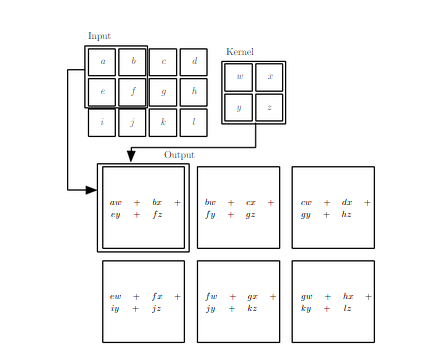
\includegraphics[width=4in]{fig/chap9/9_1.png} 
   \caption{图9.1演示了一个在2维张量上的卷积运算(核没有翻转)的例子。}
   \label{fig:9_1}
\end{figure}


离散卷积可以看作矩阵的乘法,然而,这个矩阵的一些元素被限制为必须和另一些元素相等。
例如对于单变量的离散卷积,矩阵的每一行都必须和上一行移动一个元素后相等。
这种矩阵叫做Toeplitz matrix。
对于二维情况,卷积对应着一个doubly block circulant matrix(二维矩阵)。
除了这些元素相等的限制以外,卷积通常对应着一个非常稀疏的矩阵(几乎所有的元素都为零)。
这是因为核通常要远小于输入的图像。任何一个使用矩阵乘法但是并不依赖矩阵结构的特殊性质的神经网络算法,都适用于卷积运算,并且不需要对神经网络做出大的修改。
典型的CNN为了更有效地处理大规模输入,确实使用了一些专门化的技巧,但这些在理论分析方面并不是严格必要的。

 
\section{动机}

卷积运算通过三个重要的思想来帮助改进机器学习系统:sparse interactions(局部感知)、parameter sharing(权值共享)、equivariant representations。
另外,卷积提供了一种处理大小可变的输入的方法。我们会在下文中依次介绍这些思想。

传统的神经网络使用矩阵乘法来建立输入与输出的连接关系。
其中,参数矩阵的每一个独立的参数都描述了每一个输入单元与每一个输出单元间的交互。
这意味着每一个输出单元与每一个输入单元都产生交互。
然而,CNN具有sparse interactions(也叫做sparse connectivity或者sparse weights)的特征。
这通过使得核的规模远小于输入的规模来实现。
举个例子,当进行图像处理时,输入的图像可能包含百万个像素点,但是我们可以通过只占用几十到上百个像素点的核来探测一些小的有意义的特征,例如图像的边缘。
这意味着我们需要存储的参数更少,不仅减少了模型的存储需求,而且提高了它的统计效率。
这也意味着为了得到输出我们只需要更少的计算量。
这些效率上的提高往往是很显著的。
如果有$m$个输入和$n$个输出,那么矩阵乘法需要$m \times n$个参数并且相应算法的时间复杂度为$O(m\times n)$(对于每一个例子)。
如果我们限制每一个输出拥有的连接数为$k$,那么稀疏的连接方法只需要$k\times n$个参数以及$O(k\times n)$的运行时间。
在很多应用方面,只需保持$k$的数量级远小于$m$,就能在机器学习的任务中取得好的表现。
sparse connectivity(局部感知)的图形化解释如图\ref{fig:chap9_area_of_effect}和图\ref{fig:chap9_receptive_field}所示。
在深度卷积网络中,处在深层的单元可能不直接地与绝大部分输入连接,如图\ref{fig:chap9_deep_receptive_field}所示。
这允许网络可以通过只描述sparse interactions的区域来高效地描述多个变量的复杂交互过程。


% fig 9.2
\begin{figure}[!htb]
\ifOpenSource
\centerline{\includegraphics{figure.pdf}}
\else
\centerline{\includegraphics{Chapter9/figures/area_of_effect}}
\fi
\captionsetup{singlelinecheck=off}
\caption[Caption for LOF]{\gls{sparse_connectivity},对每幅图从下往上看。我们强调了一个输入单元$x_3$以及在$\bm{s}$中受该单元影响的输出单元。\emph{(上)}当$\bm{s}$是由核宽度为3的卷积产生时,只有三个输出受到$\bm{x}$的影响\protect\footnotemark。\emph{(下)}当$\bm{s}$是由矩阵乘法产生时,连接不再是稀疏的,所以所有的输出都会受到$x_3$的影响。}
\label{fig:chap9_area_of_effect}
\end{figure}
 \footnotetext{译者注:译者认为此处应当是$x_3$。}
% fig 9.3
\begin{figure}[!htb]
\ifOpenSource
\centerline{\includegraphics{figure.pdf}}
\else
\centerline{\includegraphics{Chapter9/figures/receptive_field}}
\fi
\captionsetup{singlelinecheck=off}
\caption[.]{\gls{sparse_connectivity},对每幅图从上往下看。我们强调了一个输出单元$s_3$以及$\bm{x}$中影响该单元的输入单元。这些单元被称为$s_3$的\gls{receptive_field}。\emph{(上)}当$\bm{s}$是由核宽度为3的卷积产生时,只有三个输入影响$s_3$。\emph{(下)}当$\bm{s}$是由矩阵乘法产生时,连接不再是稀疏的,所以所有的输入都会影响$s_3$。}


\label{fig:chap9_receptive_field}
\end{figure}
% fig 9.4
\begin{figure}[!htb]
\ifOpenSource
\centerline{\includegraphics{figure.pdf}}
\else
\centerline{\includegraphics{Chapter9/figures/deep_receptive_field}}
\fi
\caption{处于\gls{convolutional_network}更深的层中的单元,它们的\gls{receptive_field}要比处在浅层的单元的\gls{receptive_field}更大。如果网络还包含类似\gls{stride}卷积(图\ref{fig:chap9_stride_conv})或者\gls{pooling}(\ref{sec:pooling}节)之类的结构特征,这种效应会加强。这意味着在\gls{convolutional_network}中即使是\emph{直接}连接都是很稀疏的,处在更深的层中的单元可以\emph{间接地}连接到全部或者大部分输入图像。}
\label{fig:chap9_deep_receptive_field}
\end{figure}

 
\firstgls{parameter_sharing}是指在一个模型的多个函数中使用相同的参数。
在传统的神经网络中,当计算一层的输出时,权值矩阵的每一个元素只使用一次,当它乘以输入的一个元素后就再也不会用到了。
作为\gls{parameter_sharing}的同义词,我们可以说一个网络含有\firstgls{tied_weights},因为用于一个输入的权值也会被绑定在其他的权值上。
在\gls{CNN}中,核的每一个元素都作用在输入的每一位置上(除了一些可能的边界像素,取决于对于边界的决策设计)。
卷积运算中的\gls{parameter_sharing}保证了我们只需要学习一个参数集合,而不是对于每一位置都需要学习一个单独的参数集合。
这虽然没有改变前向传播的时间(仍然是$O(k\times n)$),但它显著地把模型的存储需求降低至$k$个参数,并且$k$通常是远小于$m$的数量级。
因为$m$ 和$n$通常规模很接近,$k$在实际中相对于$m\times n$是很小的。
因此,卷积在存储需求和统计效率方面极大地优于稠密矩阵的乘法运算。
图\ref{fig:chap9_parameter_sharing}演示了\gls{parameter_sharing}是如何实现的。
% fig 9.5
\begin{figure}[!htb]
\ifOpenSource
\centerline{\includegraphics{figure.pdf}}
\else
\centerline{\includegraphics{Chapter9/figures/parameter_sharing}}
\fi
\caption{\gls{parameter_sharing}。黑色箭头表示在两个不同的模型中使用了特殊参数的连接。\emph{(上)}黑色箭头表示在卷积模型中3元素核的中间元素的使用。因为\gls{parameter_sharing},这单个参数被用于所有的输入位置。\emph{(下)}这单个黑色箭头表示在全连接模型中权重矩阵的中间元素的使用。这个模型没有使用\gls{parameter_sharing},所以参数只使用了一次。}
\label{fig:chap9_parameter_sharing}
\end{figure}
% -- 326 --
 
% -- 327 --
 
作为前两条原则的一个实际例子,图\ref{fig:chap9_efficiency_of_edge_detection}说明了\gls{sparse_connectivity}和\gls{parameter_sharing}是如何显著地提高用于图像边缘检测的线性函数的效率的。
% fig 9.6
\begin{figure}
\ifOpenSource
\centerline{\includegraphics{figure.pdf}}
\else
\centering    
\subfigure{ \label{fig:chap9_efficiency_of_edge_detection_a}     
\includegraphics[width=0.35\textwidth]{Chapter9/figures/sundance.png}}     
\subfigure{ \label{fig:chap9_efficiency_of_edge_detection_b}     
\includegraphics[width=0.35\textwidth]{Chapter9/figures/edges.png}}     
\fi
\captionsetup{singlelinecheck=off}
\caption{边缘检测的效率。右边的图像是通过获得原始图像中的每个像素并减去左边相邻像素的值而形成的。这给出了输入图像中所有垂直方向上的边缘的强度,这对目标检测是有用的操作。两个图像都是280像素的高度。输入图像宽320像素,而输出图像宽319像素。这个变换可以通过包含两个元素的卷积核来描述,并且需要$319\times 280\times 3 = 267,960$个浮点运算(每个输出像素需要两次乘法和一次加法)。为了用矩阵乘法描述相同的变换,需要$320\times 280\times 319\times 280$个或者说超过80亿个元素的矩阵,这使得卷积对于表示这种变换更有效40亿倍。直接运行矩阵乘法的算法将执行超过160亿个浮点运算,这使得卷积在计算上大约有60,000倍的效率。当然,矩阵的大多数元素将为零。如果我们只存储矩阵的非零元,则矩阵乘法和卷积都需要相同数量的浮点运算来计算。矩阵仍然需要包含$2\times 319\times 280=178,640$个元素。将小的局部区域上的相同线性变换应用到整个输入上,卷积是描述这种变换的极其有效的方法。照片来源:Paula Goodfellow。}   
\label{fig:chap9_efficiency_of_edge_detection}     
\end{figure}
 
对于卷积,权值的特殊形式使得神经网络层具有平移不变性。
如果一个函数满足输入改变,输出也以同样的方式改变这一性质,我们就说它是等变(equivariant)的。
特别地,如果函数$f(x)$与$g(x)$满足$f(g(x))= g(f(x))$,我们就说$f(x)$对于变换$g$具有等变性。
对于卷积来说,如果令$g$是任意的输入平移函数,那么卷积函数对于$g$具有等变性。
举个例子,令$I$表示图像的明亮度函数(取值为整数),$g$表示图像函数的变换函数(把一个图像函数映射到另一个图像函数的函数)使得$I' = g(I)$,其中$I'(x,y) = I(x-1, y)$。
这个函数把$I$中的每个像素向右移动一格。
如果我们先对$I$进行这种变换然后进行卷积操作所得到的结果,与先对$I$进行卷积然后再对输出使用平移函数$g$得到的结果是一样的。
当处理时间序列数据时,卷积产生一条用来表明输入中出现不同特征的某种时间轴。
如果我们把输入中的一个事件向后延时,在输出中也会有完全相同的表示,只是时间延时了。
图像与之类似,卷积产生了一个2维映射来表明某种属性在输入的什么位置出现了。
如果我们移动输入中的对象,它的表示也会在输出中移动同样的量。
当处理多个输入位置时,一些作用在邻居像素的函数是很有用的。
例如在处理图像时,在CNN的第一层进行图像的边缘检测是很有用的。
相同的边缘或多或少地散落在图像的各处,所以应当对整个图像有权值共享
但在某些情况下,我们并不希望对整幅图共享权值。
例如当我们在处理人脸图像(图像已经被剪裁成人脸在中心)时,我们可能会希望在不同的部位探测出不同的特征(处理人脸上部的网络需要去搜寻眉毛,处理人脸下部的网络就需要去搜寻下巴了)。

 
卷积对其他的一些变换并不是天然等变的,例如对于图像尺度或者角度的变换,需要其他的一些机制来处理这些变换。

最后,一些不能被传统的由(固定大小的)矩阵乘法定义的神经网络处理的特殊数据,可能通过卷积神经网络来处理,我们将在\ref{sec:data_types}节中进行讨论。

\section{pooling}

卷积神经网络的卷积层通常包含三级(如图\ref{fig:chap9_conv_layer}所示)。
在第一级中,卷积层并行地进行多个卷积运算来产生一组线性激活函数。
在第二级中,非线性的激活函数如ReLU函数等作用在第一级中的每一个线性输出上。
这一级有时也被称为detector stage(检测阶段?)。
在第三级中,我们使用pooling funciton函数(下采样函数)来更进一步地调整卷积层的输出。


% fig 9.7
\begin{figure}[!htb]
\ifOpenSource
\centerline{\includegraphics{figure.pdf}}
\else
\centerline{\includegraphics{Chapter9/figures/conv_layer}}
\fi
\caption{典型\gls{CNN}层的组件。有两组常用的术语用于描述这些层。\emph{(左)}在这组术语中,\gls{convolutional_network}被视为少量相对复杂的层,每层具有许多``级''。在这组术语中,核张量与网络层之间存在一一对应关系。在本书中,我们通常使用这组术语。\emph{(右)}在这组术语中,\gls{convolutional_network}被视为更大数量的简单层;每一个处理步骤都被认为是一个独立的层。这意味着不是每个``层''都有参数。}
\label{fig:chap9_conv_layer}
\end{figure}

pooling函数(下采样层)使用某一位置的相邻输出的总体统计特征来代替网络在该位置的输出。
例如,max pooling函数给出相邻矩形区域内的最大值。
其他常用的pooling函数包括相邻矩形区域内的平均值、$L^2$范数以及依靠据中心像素距离的加权平均函数。

 
不管采用什么样的pooling函数,当输入作出少量平移时,pooling能帮助我们的表示近似不变的。
对于平移的不变性是说当我们把输入平移一微小的量,大多数通过pooling函数的输出值并不会发生改变。
图\ref{fig:chap9_max_pool_invariance}用了一个例子来说明这是如何实现的。
局部平移不变性是一个很重要的性质,尤其是当我们关心某个特征是否出现而不关心它出现的具体位置时。
例如,当判定一张图像中是否包含人脸时,我们并不需要知道眼睛的具体像素位置,我们只需要知道有一只眼睛在脸的左边,有一只在右边就行了。
但在一些其他领域,保存特征的具体位置却很重要。
例如当我们想要寻找一个由两条边相交而成的拐角时,我们就需要很好地保存边的位置来判定它们是否相交。

% fig 9.8
\begin{figure}[!htb]
\ifOpenSource
\centerline{\includegraphics{figure.pdf}}
\else
\centerline{\includegraphics{Chapter9/figures/max_pool_invariance}}
\fi
\caption{\gls{max_pooling}引入不变性。\emph{(上)}卷积层中间输出的视图。下面一行显示非线性的输出。上面一行显示\gls{max_pooling}的输出,每个\gls{pool}的宽度为三个像素并且\gls{pooling}区域的\gls{stride}为一个像素。\emph{(下)}相同网络的视图,不过对输入右移了一个像素。下面一行的所有值都发生了改变,但上面一行只有一半的值发生了改变,这是因为\gls{max_pooling}单元只对周围的最大值比较敏感,而不是对精确的位置。}
\label{fig:chap9_max_pool_invariance}
\end{figure}

 
使用pooling可以认为网络结构中增加了一个无限强的先验:卷积层学得的函数必须具有对少量平移的不变性。当这个假设成立时,pooling可以极大地提高网络的统计效率。

pooling对于空间区域具有平移不变性,但当我们对于分离参数的卷积输出进行pooling操作时,特征能够学得应该对于哪种变换具有不变性(如图\ref{fig:chap9_learned_rotation}所示)。


% fig 9.9
\begin{figure}[!htb]
\ifOpenSource
\centerline{\includegraphics{figure.pdf}}
\else
\centerline{\includegraphics{Chapter9/figures/learned_rotation}}
\fi
\caption{学习不变性的示例。使用分离的参数学得多个特征,再使用\gls{pooling}单元进行\gls{pooling},可以学得对输入的某些变换的不变性。这里我们展示了用三个学得的过滤器和一个\gls{max_pooling}单元可以学得对旋转变换的不变性。这三个过滤器都旨在检测手写的数字5。每个过滤器尝试匹配稍微不同方向的5。当输入中出现5时,相应的过滤器会匹配它并且在探测单元中引起大的激活。然后,无论哪个探测单元被激活,\gls{max_pooling}单元都具有大的激活。我们在这里展示网络如何处理两个不同的输入,导致两个不同的探测单元被激活。然而对\gls{pooling}单元的影响大致相同。这个原则在\gls{maxout}网络\citep{Goodfellow-et-al-ICML2013}和其他卷积网络中使用。空间位置上的\gls{max_pooling}对于平移是天然不变的;这种多通道方法只在学习其他变换时是必要的。}
\label{fig:chap9_learned_rotation}
\end{figure}

 
因为pooling总结了全部的周围邻居的反馈,这使得pooling单元少于探测单元成为可能,我们可以通过综合pooling区域的$k$个像素的统计特征而不是单个像素来实现。
图\ref{fig:chap9_pool_downsample}给出了一个例子。
这种方法提高了网络的计算效率,因为下一层少了约$k$ 倍的输入。
当下一层的参数数目是其输入大小的函数时(例如当下一层是全连接的依赖矩阵乘法的网络层时),这种对于输入规模的减小也可以提高统计效率并且减少对于参数的存储需求。


% fig 9.10
\begin{figure}[!htb]
\ifOpenSource
\centerline{\includegraphics{figure.pdf}}
\else
\centerline{\includegraphics{Chapter9/figures/pool_downsample}}
\fi
\caption{带有\gls{downsampling}的\gls{pooling}。这里我们使用\gls{max_pooling},\gls{pool}的宽度为三并且\gls{pool}之间的\gls{stride}为二。这使得表示的大小减少了一半,减轻了下一层的计算和统计负担。注意到最右边的\gls{pooling}区域尺寸较小,但如果我们不想忽略一些探测单元的话就必须包含这个区域。}
\label{fig:chap9_pool_downsample}
\end{figure}

 
在很多任务中,pooling对于处理不同大小的输入具有重要作用。
例如我们想对不同大小的图像进行分类时,分类层的输入必须是固定的大小,而这通常通过调整pooling区域的偏置大小来实现,这样分类层总是能接收到相同数量的统计特征而不管最初的输入大小了。
例如,最终的pooling层可能会输出四组综合统计特征,每组对应着图像的一个象限,而与图像的大小无关。

一些理论工作对于在不同情况下应当使用哪种pooling函数给出了一些指导。
动态地把特征pooling在一起也是可行的,例如,通过针对具有特定性质的位置运行聚类算法。
这种方法对于每幅图像产生一个不同的pooling区域集合。
另一种方法是先学习一个单独的pooling结构,再应用到全部的图像中。

pooling可能会使得一些利用自顶向下信息的神经网络结构变得复杂,例如玻尔兹曼机和稀疏自编码器。
这些问题将在第\ref{part:deep_learning_research}部分中当我们遇到这些类型的网络时进一步讨论。
convolutional Boltzmann machines 中的\gls{pooling}出现在\ref{sec:convolutional_boltzmann_machines}节。
一些可微网络中需要的在{pooling单元中进行的类逆运算将在\ref{sec:convolutional_generative_networks}节中讨论。

图\ref{fig:chap9_cnn_classifier}给出了一些使用卷积和\gls{pooling}操作的用于分类的\gls{CNN}的完整结构的例子。
% fig 9.11
\begin{figure}[!htb]
\ifOpenSource
\centerline{\includegraphics{figure.pdf}}
\else
\centerline{\includegraphics{Chapter9/figures/cnn_classifier}}
\fi
\caption{\gls{convolutional_network}用于分类的架构示例。本图中使用的具体\gls{stride}和深度并不适合实际使用;它们被设计得非常浅以适合页面。实际的\gls{convolutional_network}也常常涉及大量的分支,不同于这里为简单起见所使用的链式结构。\emph{(左)}处理固定大小的图像的\gls{convolutional_network}。在卷积层和\gls{pooling}层几层交替之后,卷积特征映射的张量被重新整形以展平空间维度。网络的其余部分是一个普通的前馈网络分类器,如第\ref{chap:deep_feedforward_networks}章所述。\emph{(中)}处理大小可变的图像的\gls{convolutional_network},但仍保持全连接的部分。该网络使用具有可变大小但是数量固定的\gls{pool}的\gls{pooling}操作,以便向网络的全连接部分提供576个单位的固定大小的向量。 \emph{(右)}没有任何全连接权重层的\gls{convolutional_network}。相反,最后的卷积层为每个类输出一个特征映射。该模型可能学习每个类在每个空间位置出现的可能性的映射。将特征映射进行平均得到的单个值,提供了顶部softmax分类器的变量。}
\label{fig:chap9_cnn_classifier}
\end{figure}

\section{卷积与\glsentrytext{pooling}作为一种无限强的先验}


回忆一下\ref{sec:capacity_overfitting_and_underfitting}节中prior probability distribution(先验概率分布)的概念。

这是一个模型参数的概率分布,它表示在我们了解数据之前我们假设数据是处于什么分布。

 
先验被认为是强或者弱取决于先验中概率密度的集中程度。
弱先验具有较高的熵值,例如方差很大的gaussian distribution,这样的先验允许数据对于参数的改变具有或多或少的自由性。
强先验具有较低的熵值,例如方差很小的gaussian distribution,这样的先验在决定参数最终取值时起着更加积极的作用。

一个无限强的先验对一些参数的概率置零并且要求禁止对这些参数赋值,无论数据对于这些参数的值给出了多大的支持。

我们可以把CNN想成和全连接网络类似,但对于这个全连接网络的权值有一个无限强的先验。
这个无限强的先验是说一个隐藏神经元的权值必须和它邻居的权值相等,但在空间中改变。
这个先验也要求除了那些处在神经元空间连续的小的接收域以内的权值外,其余的权值都为零。

总之,我们可以把卷积的使用当作是对网络中一层的参数引入了一个无限强的先验概率分布。
这个先验是说该层应该学得的函数只包含局部连接关系并且对平移具有等变性。
类似的,使用下采样层也是一个无限强的先验:每一个单元都具有对少量平移的不变性。

当然,把CNN当作一个具有无限强先验的全连接网络来实现会导致极大的计算浪费。
但把CNN想成具有无限强先验的全连接网络可以帮助我们更好地理解CNN是如何工作的。

其中一个关键的地方是卷积和pooling可能导致欠拟合。
与任何其他先验类似,卷积和pooling只有当先验的假设合理且正确时才有用。

如果一项任务依赖于保存精确的空间信息,那么在所有的特征上使用pooling将会增大训练误差。
一些CNN\citep{Szegedy-et-al-arxiv2014}为了既获得具有较高不变性的特征又获得当平移不变性不合理时不会导致欠拟合的特征,被设计成在一些通道上使用\gls{pooling}而在另一些通道上不使用。
当一项任务涉及到要对输入中相隔较远的信息进行合并时,那么卷积所需要的先验可能就不正确了。

另一个关键洞察是当我们比较卷积模型的统计学习表现时,只能以基准中的其他卷积模型作为比较的对象。
其他不使用卷积的模型即使我们把图像中的所有像素点都置换后依然有可能进行学习。
对于许多图像数据集,还有一些分别的基准,有些是针对那些具有\firstgls{permutation_invariant}并且必须通过学习发现拓扑结构的模型,还有一些是针对设计者将空间关系的知识通过硬编码给了它们的模型。

% -- 336 --

\section{基本卷积函数的变体}
\label{sec:variants_of_the_basic_convolution_function}

当在神经网络的上下文中讨论卷积时,我们通常不是特指数学文献中使用的那种标准的离散卷积运算。
实际应用中的函数略微有些不同。
这里我们详细讨论一下这些差异,并且对神经网络中用到的函数的一些重要性质进行重点说明。

首先,当我们提到神经网络中的卷积时,我们通常是指一次特定的运算,而这种运算包含了并行地使用多个卷积。
这是因为带有单个核的卷积只能提取一种类型的特征,尽管它作用在多个空间位置上。
我们通常希望神经网络的一层能够在多个位置提取多种类型的特征。

另外,输入通常也不仅仅是实值的网格,而是由一系列向量值的观测数据构成的网格。
例如,一幅彩色图像在每一个像素点都会有红绿蓝三种颜色的亮度。
在多层的CNN中,第二层的输入是第一层的输出,通常在每个位置包含多个卷积的输出。
当用于图像时,我们通常把卷积的输入输出都看作是3维的张量,其中一个索引用于标明不同的通道(例如红绿蓝),另外两个索引标明在每个通道上的空间坐标。
软件实现通常使用批处理模式,所以它们会使用4维的张量,第四维索引用于标明批处理中不同的实例,但我们为简明起见这里忽略批处理索引。

因为CNN通常使用多通道的卷积,它们基于的线性运算并不保证一定是可交换的,即使使用了核翻转也是如此。
这些多通道的运算只有当其中的每个运算的输出和输入具有相同的通道数时才是可交换的。

假定我们有一个4维的核张量$\TSK$,它的每一个元素是$\TEK_{i,j,k,l}$,表示输出的处于通道$i$中的一个单元和输入的处于通道$j$中的一个单元的连接强度,并且在输出单元和输入单元之间有一个$k$行$l$列的偏置。

假定我们的输入由观测数据$\TSV$组成,它的每一个元素是$\TEV_{i,j,k}$,表示处在通道$i$中第$j$行第$k$列的值。

假定我们的输出$\TSZ$和输入$\TSV$具有相同的形式。如果输出$\TSZ$是通过对$\TSK$和$\TSV$进行卷积而不涉及翻转$\TSK$得到的,那么

\begin{equation}
\TEZ_{i,j,k} = \sum_{l,m,n} \TEV_{l, j+m-1, k+n-1} \TEK_{i,l,m,n},
\end{equation}

这里对所有的$l$,$m$和$n$进行求和是对所有(在求和式中)有效的张量索引的值进行求和。
在线性代数中,向量的索引通常从1开始,这就是上述公式中$-1$的由来。
但是像C或Python这类编程语言索引通常从0开始,这使得上述公式可以更加简洁。

 
我们有时会希望跳过核中的一些位置来降低计算的开销(相应的代价是提取特征没有先前那么好了)。
我们可以把这一过程看作是对卷积函数输出的下采样(downsampling)。
如果我们只想对输出的每个方向上的$s$个像素进行采样,那么我们可以定义一个下采样卷积函数$c$使得
\begin{equation}
\TEZ_{i,j,k} = c(\TSK, \TSV, s)_{i,j,k} = \sum_{l,m,n} [\TEV_{l,(j-1)\times s+m, (k-1)\times s +n,}
 \TEK_{i,l,m,n}].
 \label{eq:9.8}
\end{equation}
我们把$s$称为下采样卷积的stride(步长)。
当然也可以对每个移动方向定义不同的步幅。
图\ref{fig:chap9_stride_conv}演示了一个实例。
% fig 9.12
\begin{figure}[!htb]
\ifOpenSource
\centerline{\includegraphics{figure.pdf}}
\else
\centerline{\includegraphics{Chapter9/figures/stride_conv}}
\fi
\caption{带有\gls{stride}的卷积。在这个例子中,我们的\gls{stride}为二。\emph{(上)}在单个操作中实现的\gls{stride}为二的卷积。\emph{(下)}\gls{stride}大于一个像素的卷积在数学上等价于单位\gls{stride}的卷积随后\gls{downsampling}。显然,涉及\gls{downsampling}的两步法在计算上是浪费的,因为它计算了许多将被丢弃的值。}
\label{fig:chap9_stride_conv}
\end{figure}

在任何CNN的应用中都有一个重要性质,那就是能够隐含地对输入$\TSV$用零进行填充(pad)使得它加宽。
如果没有这个性质,表示的宽度在每一层就会缩减,缩减的幅度是比核少一个像素这么多。
对输入进行零填充允许我们对核的宽度和输出的大小进行独立的控制。
如果没有零填充,我们就被迫面临二选一的局面,要么选择网络空间宽度的快速缩减,要么选择一个小型的核——这两种情境都会极大得限制网络的表示能力。

图\ref{fig:chap9_zero_pad_shrink}给出了一个例子。
% fig 9.13
\begin{figure}[!htb]
\ifOpenSource
\centerline{\includegraphics{figure.pdf}}
\else
\centerline{\includegraphics{Chapter9/figures/zero_pad_shrink}}
\fi
\caption{零填充对网络大小的影响。考虑一个\gls{convolutional_network},每层有一个宽度为六的核。 在这个例子中,我们不使用任何\gls{pooling},所以只有卷积操作本身缩小网络的大小。\emph{(上)}在这个卷积网络中,我们不使用任何隐含的零填充。这使得表示在每层缩小五个像素。从十六个像素的输入开始,我们只能有三个卷积层,并且最后一层不能移动核,所以可以说只有两层是真正的卷积层。可以通过使用较小的核来减缓收缩速率,但是较小的核表示能力不足,并且在这种结构中一些收缩是不可避免的。\emph{(下)}通过向每层添加五个隐含的零,我们防止了表示随深度收缩。这允许我们设计一个任意深的卷积网络。}
\label{fig:chap9_zero_pad_shrink}
\end{figure}

有三种零填充设定的情况值得注意。
第一种是无论怎样都不使用零填充的极端情况,并且卷积核只允许访问那些图像中能够完全包含整个核的位置。
在MATLAB中,这称为valid卷积。

在这种情况下,输出的所有像素都是输入中相同数量像素的函数,这使得输出像素的表示更加规范。
然而,输出的大小在每一层都会缩减。
如果输入的图像宽度是$m$,核的宽度是$k$,那么输出的宽度就会变成$m-k+1$。
如果卷积核非常大的话缩减率会非常显著。
因为缩减数大于0,这限制了网络中能够包含的卷积层的层数。
当层数增加时,网络的空间维度最终会缩减到$1\times 1$,这种情况下另外的层就不可能进行有意义的卷积了。
第二种特殊的情况是只进行足够的零填充来保持输出和输入具有相同的大小
。
在MATLAB中,这称为same卷积。
在这种情况下,网络能够包含任意多的卷积层,只要硬件可以支持,这是因为卷积运算并没有改变相关的结构。
然而,输入像素中靠近边界的部分相比于中间部分对于输出像素的影响更小。
这可能会导致边界像素存在一定程度的欠表示。
这使得第三种极端情况产生了,在MATLAB中称为full卷积。

它进行了足够多的零填充使得每个像素在每个方向上恰好被访问了$k$次
这将导致学得一个在卷积特征映射的所有位置都表现不错的单核更为困难。
通常零填充的最优数量(对于测试集的分类正确率)处于``valid卷积''和``same卷积''之间的某个位置。



在一些情况下,我们并不一定真正想用卷积,而只是用一些局部连接的网络层。
在这种情况下,我们的多层感知机对应的邻接矩阵是相同的,但每一个连接都有它自己的权重,用一个6维的张量$\TSW$来表示。
$\TSW$的索引分别是:输出的通道$i$,输出的行$j$和列$k$,输入的通道$l$,输入的行偏置$m$和列偏置$n$。
局部连接层的线性部分可以表示为

\begin{equation}
\TEZ_{i,j,k} = \sum_{l,m,n} [\TEV_{l, j+m-1, k+n-1} w_{i, j, k, l, m, n}]. %这里应该是$\TEW$?,不清楚,待考证
\end{equation}
这有时也被称为unshared convolution(非权值共享的卷积?),因为它和带有一个小核的离散卷积运算很像,但并不横跨位置来共享参数。
图\ref{fig:chap9_local}比较了局部连接、卷积和全连接的区别。


% fig 9.14
\begin{figure}[!htb]
\ifOpenSource
\centerline{\includegraphics{figure.pdf}}
\else
\centerline{\includegraphics{Chapter9/figures/local}}
\fi
\caption{局部连接,卷积和全连接的比较。\emph{(上)}每一小片(接受域)有两个像素的局部连接层。每条边用唯一的字母标记,来显示每条边都有自身的权重参数。\emph{(中)}核宽度为两个像素的卷积层。该模型与局部连接层具有完全相同的连接。区别不在于哪些单元相互交互,而在于如何共享参数。局部连接层没有\gls{parameter_sharing}。卷积层在整个输入上重复使用相同的两个权重,正如用于标记每条边的字母重复出现所指示的那样。\emph{(下)}全连接层类似于局部连接层,它的每条边都有其自身的参数(在该图中用字母明确标记的话就太多了)。 然而,它不具有局部连接层的连接受限的特征。}
\label{fig:chap9_local}
\end{figure}
 

 
当我们知道每一个特征都是一小部分空间的函数而不是整个空间的特征时,局部连接层是很有用的。
例如,如果我们想要辨别一张图片是否是人脸图像时,我们只需要去寻找嘴是否在图像的下部中央部分即可。

使用那些连接被更进一步限制的卷积或者局部连接层也是有用的,例如,限制每一个输出的通道$i$仅仅是输入通道$l$的一部分的函数时。
实现这种情况的一种通用方法是使输出的前$m$个通道仅仅连接到输入的前$n$个通道,输出的接下来的$m$个通道仅仅连接到输入的接下来的$n$个通道,以此类推。


图\ref{fig:chap9_conv_groups}给出了一个例子。
对少量通道间的连接进行建模允许网络使用更少的参数,这降低了存储的消耗以及提高了统计效率,并且减少了前向和反向传播所需要的计算量。
这些目标的实现并没有减少隐藏神经元的数目。


% fig 9.15
\begin{figure}[!htb]
\ifOpenSource
\centerline{\includegraphics{figure.pdf}}
\else
\centerline{\includegraphics{Chapter9/figures/conv_groups}}
\fi
\caption{\gls{convolutional_network}的前两个输出通道只和前两个输入通道相连,随后的两个输出通道只和随后的两个输入通道相连。}
\label{fig:chap9_conv_groups}
\end{figure}

tiled convolution对卷积层和局部连接层进行了折衷。
这里并不是对每一个空间位置的权重集合进行学习,我们学习一组核使得当我们在空间移动时它们可以循环利用。
这意味着在近邻的位置上拥有不同的过滤器,就像局部连接层一样,但是对于这些参数的存储需求仅仅会增长常数倍,这个常数就是核的集合的大小,而不是整个输出的特征映射的大小。


图\ref{fig:chap9_tiled}对局部连接层、tiled convolution和标准卷积进行了比较。
% fig 9.16
\begin{figure}[!htb]
\ifOpenSource
\centerline{\includegraphics{figure.pdf}}
\else
\centerline{\includegraphics{Chapter9/figures/tiled}}
\fi
\captionsetup{singlelinecheck=off}
\caption[.]{局部连接层、\gls{tiled_convolution}和标准卷积的比较。当使用大小相同的核时,这三种方法的单元之间具有相同的连接。此图是对使用两个像素宽的核的说明。这三种方法之间的区别在于它们如何共享参数。\emph{(上)}局部连接层根本没有共享参数。我们对每个连接使用唯一的字母标记,来表明每个连接都有它自身的权重。\emph{(中)}\gls{tiled_convolution}有$t$个不同的核。这里我们说明$t=2$的情况。其中一个核具有标记为``a''和``b''的边,而另一个具有标记为``c''和``d''的边。我们每次在输出中向右移动一个像素,移动后使用不同的核。这意味着,与局部连接层类似,输出中的相邻单元具有不同的参数。与局部连接层不同的是,在我们遍历所有可用的$t$个核之后,我们循环回到了第一个核。如果两个输出单元间隔$t$个步长的倍数,则它们共享参数。\emph{(下)}传统卷积等效于$t=1$的\gls{tiled_convolution}。它只有一个核,并且被应用到各个地方,我们在图中表示为在各处使用具有标记为``a''和``b''的边的核。}
\label{fig:chap9_tiled}
\end{figure}
 

 
为了代数地定义tiled convolution},令$\TSK$是一个6维的张量
我们这里并不是使用分别的索引来表示输出映射中的每一个位置,输出的位置在每个方向上在$t$个不同的核的组成的集合中进行循环。
如果$t$等于输出的宽度,这就是局部连接层了。

\begin{equation}
\TEZ_{i, j, k} = \sum_{l, m, n} \TEV_{l, j+m-1, k+n-1} \TEK_{i, l, m, n, j\% t +1, k\% t+1},
\end{equation}
这里百分号是取模运算,其中$t\% t =0, (t+1)\% t = 1$等等。
在每一维上使用不同的$t$可以很直观地对这个公式进行扩展。
 

 
局部连接层与tiled convolution层都和max pooling有一些关联:这些层的探测单元都是由不同的滤波器产生的。
如果这些过滤器能够学会探测相同隐含特征的不同变换形式,那么max_pooling的单元对于学得的变换就具有不变性(如图\ref{fig:chap9_learned_rotation}所示)。
卷积层对于平移具有内置的不变性。
 

 
实现CNN时,采用除卷积以外一般要进行其他的操作。
为了实现学习,必须在给定输出的梯度时能够计算核的梯度。
在一些简单情况下,这种运算可以通过卷积来实现,但在很多我们感兴趣的情况下,包括stride大于1的情况,并不具有这样的性质。

由于卷积是一种线性运算,所以可以表示成矩阵乘法的形式(如果我们首先把输入张量变形为一个扁平的向量)。涉及到的矩阵是卷积核的函数。
这个矩阵是稀疏的并且核的每个元素都复制给矩阵的很多个元素。
这种观点能够帮助我们导出CNN需要的很多其他运算。

通过卷积定义的矩阵转置的乘法就是这样一种运算。
这种运算用于通过卷积层反向传播误差的导数,所以它在训练多于一个隐藏层的CNN时是必要的。
如果我们想要从隐藏层单元重构可视化单元时,同样的运算也是需要的。
重构可视化单元是本书第\ref{part:deep_learning_research}部分的模型广泛用到的一种运算,这些模型包括稀疏自编码器,限制玻尔兹曼机和稀疏编码等等。


构建这些模型的卷积化的版本都要用到转置化卷积。
就像核梯度的运算,这种输入梯度运算在某些情况下可以用卷积来实现,但在一般情况下需要用到第三种运算来实现。
必须非常小心地来使这种转置运算和前向传播过程相协调。
转置运算返回的输出的大小取决于三个方面:零填充的策略、前向传播运算的步长和前向传播的输出映射的大小。
在一些情况下,不同大小的输入通过前向传播过程能够得到相同大小的输出映射,所以必须明确地告知转置运算原始输入的大小。

这三种运算——卷积、从输出到权重的反向传播和从输出到输入的反向传播——对于训练任意深度的前馈卷积网络,以及训练带有(基于卷积的转置的)重构函数的卷积网络,这三种运算都足以计算它们所需的所有梯度。

对于完全一般的多维、多样例情况下的公式,完整的推导可以参见\cite{Goodfellow-TR2010}。 
为了直观说明这些公式是如何起作用的,我们这里给出一个二维单个样例的版本。
 

 
假设我们想要训练这样一个CNN,它包含步长为$s$的卷积,该卷积的核为$\TSK$,作用于多通道的图像$\TSV$,表示为$c(\TSK, \TSV, s)$,就像公式\ref{eq:9.8}中一样。
假设我们想要优化某个损失函数$J(\TSV, \TSK)$。
在前向传播过程中,我们需要用$c$本身来输出$\TSZ$,然后$\TSZ$传递到网络的其余部分并且被用来计算损失函数$J$。
在反向传播过程中,我们会收到一个张量$\TSG$表示为$\TEG_{i, j, k} = \frac{\partial}{\partial \TEZ_{i, j, k}} J(\TSV, \TSK)$。

为了训练网络,我们需要对卷积核中的权重求导。
为了实现这个目的,我们使用一个函数

\begin{equation}
g(\TSG, \TSV, s)_{i, j, k, l} = \frac{\partial}{\partial \TEK_{i, j, k, l}} J(\TSV, \TSK) = \sum_{m, n} \TEG_{i, m, n} \TEV_{j, (m-1)\times s+k, (n-1)\times s+l}.
\end{equation}

如果这一层不是网络的最后一层,我们需要对$\TSV$求梯度来使得误差进一步反向传播。
我们可以使用如下的函数

\begin{eqnarray}
h(\TSK, \TSG, s)_{i, j, k} &=& \frac{\partial }{\partial \TEV_{i, j, k}} J(\TSV, \TSK)\\
&=& \sum_{\substack{l, m\\
                  \text{s.t.}\\
                  (l-1)\times s+m = j}} \sum_{\substack{n, p\\
                                                            \text{s.t.}\\
                                                            (n-1)\times s +p = k}}
            \sum_q \TEK_{q,i,m,p} \TEG_{q, l, n}.
\end{eqnarray}


第\ref{chap:autoencoders}章描述的稀疏自编码器网络,是一些训练成把输入复制到输出的前馈网络。
一个简单的例子是PCA(主成分分析)算法,将输入$\bm{x}$拷贝到一个近似的重构值$\bm{r}$,通过函数$\bm{W}^\top \bm{Wx}$来实现。
使用权重矩阵转置的乘法,就像PCA算法这种,在一般的AE(稀疏自编码器)中是很常见的。
为了使这些模型卷积化,我们可以用函数$h$来实现卷积运算的转置。
假定我们有和$\TSZ$相同格式的隐藏单元$\TSH$,并且我们定义一种重构运算

\begin{equation}
\TSR = h(\TSK, \TSH, s).
\end{equation}

为了训练AE,我们会收到关于$\TSR$的梯度,表示为一个张量$\TSE$。
为了训练解码器,我们需要获得对于$\TSK$的梯度,通过$g(\TSH, \TSE, s)$来得到。
为了训练编码器,我们需要获得对于$\TSH$的梯度,通过$c(\TSK, \TSE, s)$来得到。
也可能通过用$c$和$h$对$g$求微分得到,但这些运算对于任何标准神经网络上的反向传播算法来说都是不需要的。
 

 
一般来说,在卷积层从输入到输出的变换中我们不仅仅只用线性运算。
我们一般也会在进行非线性运算前,对每个输出加入一些偏置项。
这样就产生了如何在偏置项中共享参数的问题。
对于局部连接层,很自然地对每个单元都给定它特有的偏置,对于tiled convolution,也很自然地用与核一样的拼接模式来共享参数。
对于卷积层来说,通常的做法是在输出的每一个通道上都设置一个偏置,这个偏置在每个卷积映射的所有位置上共享。
然而,如果输入是已知的固定大小,也可以在输出映射的每个位置学习一个单独的偏置。
分离这些偏置可能会稍稍降低模型的统计效率,但同时也允许模型来校正图像中不同位置的统计差异。
例如,当使用隐含的零填充时,图像边缘的探测单元接收到较少的输入,因此需要较大的偏置。

